\section{Theoretical foundation and governing equations}
The mathematical basis for Omnisoot is explained in the top-to-bottom hierarchical order. First, the governing equations for constant volume, constant pressure, perfectly stirred and plug flow reactor models are reviewed in Sections~\ref{sec:cvr}-\ref{sec:pfr}. The transport equations of ``soot variables" include the source terms that account for change in each soot variable due to inception, surface growth, oxidation and coagulation. Then, particle dynamics models are explained in Sections~\ref{sec:particledynamics} that entail the description of size distribution and morphology of soot particles and their collision rate, which is used to determine the coagulation source terms. Section~\ref{sec:pahgrowmodel} focuses on the \textit{``PAH growth"} models that take care of inception and adsorption from designated precursors and calculate the corresponding source terms. Similarly, the \textit{"surface reactions"} model is detailed in Section~\ref{sec:surfreacmodel}, which elaborates on the surface growth and oxidation rates based on HACA mechanism. Figure~\ref{fig:structure} illustrates the general structure of Omnisoot and its sub-models.

\begin{figure}[!htbp]
	\centering
	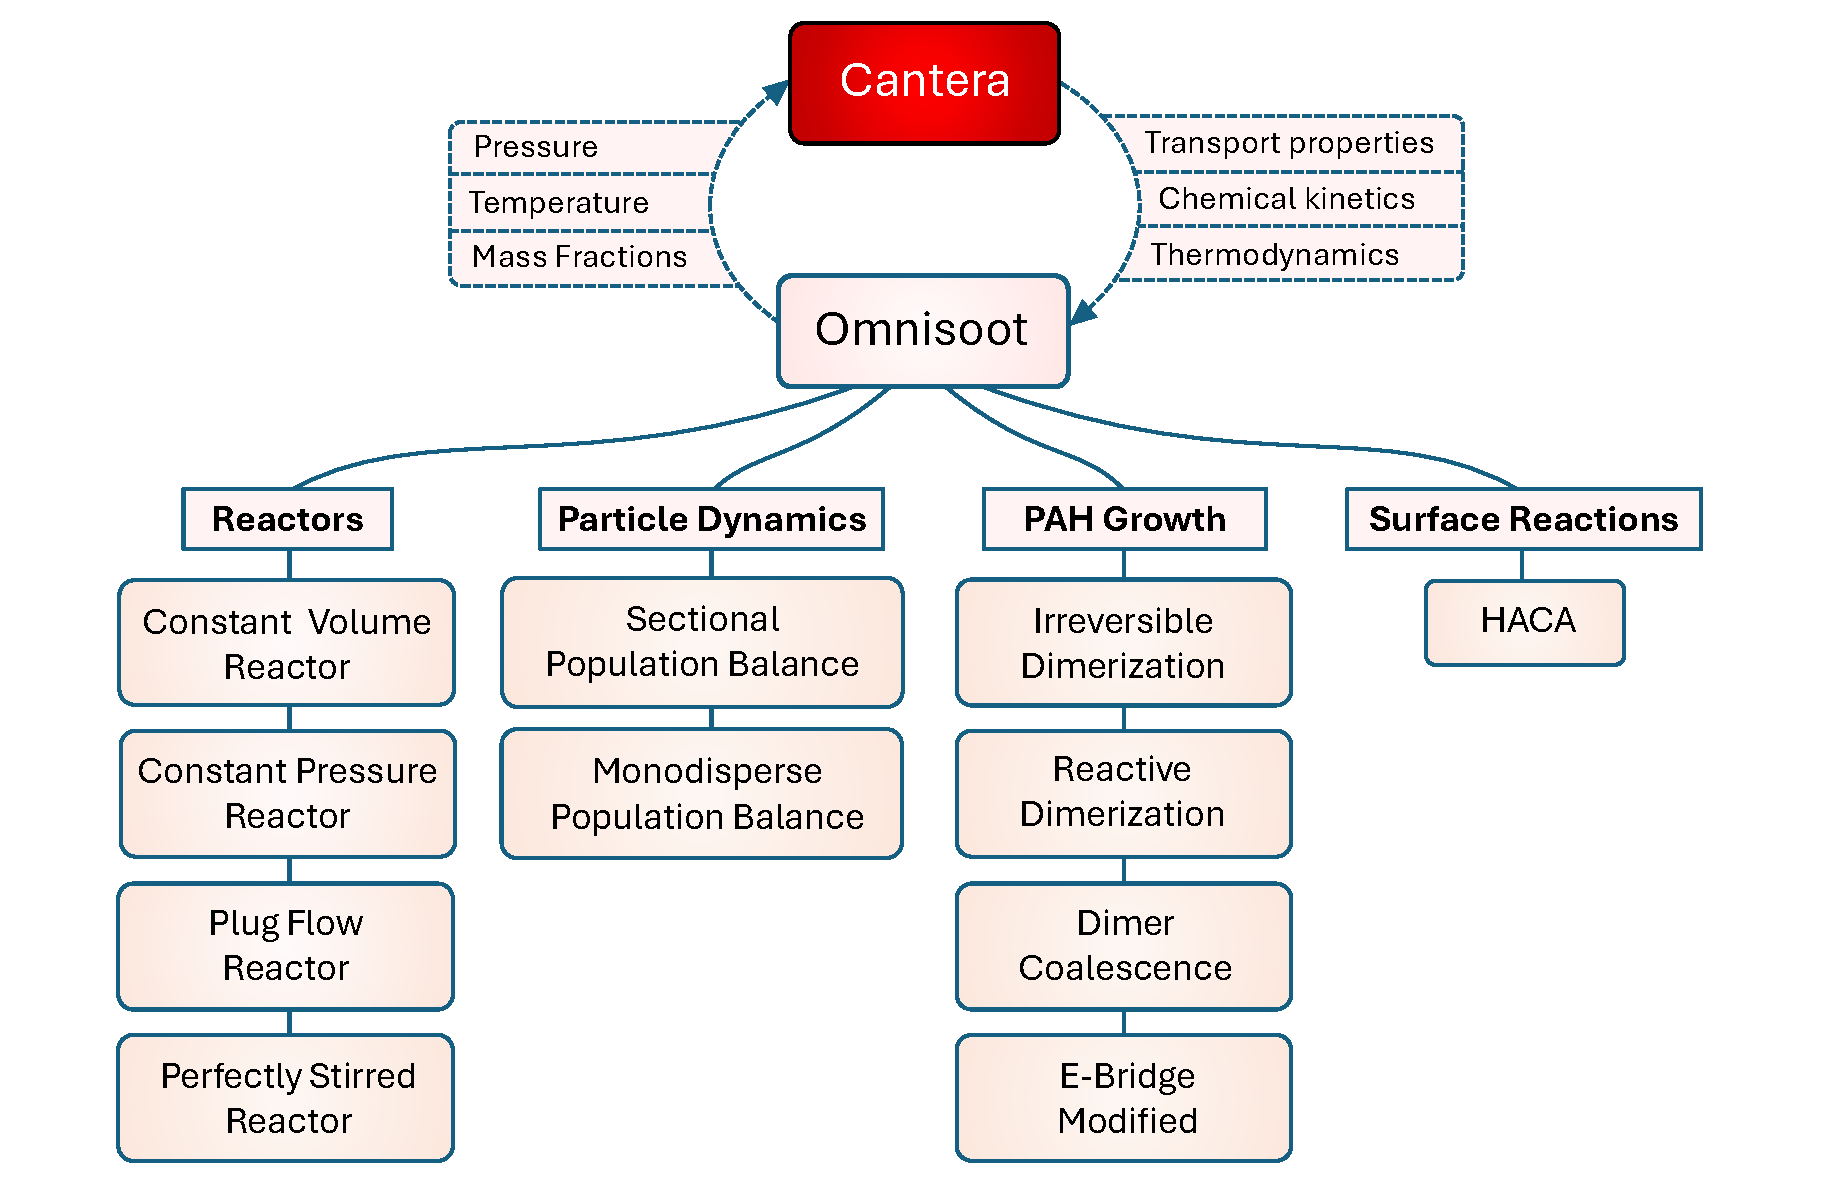
\includegraphics[height=90mm, ]{Figures/Theory/structure.pdf}
	\caption{The structure of Omnisoot that illustrates the coupling with Cantera and sub-models including the reactors, the particle dynamic models, the PAH growth models and the surface reactions model.}
	\label{fig:structure}
\end{figure}

\subsection{Assumptions and conventions}
Here, the main conventions and assumptions used in the derivation of the mathematical models are listed below.

\begin{enumerate}
%\item The ideal gas law is used to calculated physical, transport, and chemical properties of gas mixtures.

\item $f_v$ and $\varphi$ denote the volume of soot particles normalized by the gas volume and reactor volume, respectively. Their relationship can be expressed as:

\begin{equation}
	\begin{split}
		f_v = \frac{V_{soot}}{V_{gas}}, \\
		\varphi = \frac{V_{soot}}{V_{gas} + V_{soot}}, \\
		\varphi = \frac{f_v}{1 + f_v}
		\label{eqn:fvdef}.
	\end{split}
\end{equation}

\item ${\dot{s}_k}$ denotes the rate production/consumption of $k_{th}$ gaseous species (i.e., gas scrubbing) due to soot inception, surface growth and oxidation. It is positive when the species is released to the gas mixture.

\item Each soot agglomerate consists of monodisperse spherical primary particles, which are in point contact. So, the model does not consider formation of necking (or sintering) in soot agglomerates by surface growth.

%\item The primary particles of each agglomerate are similar enough that can be described by mean size and composition.

\item The word \textit{``particle"} refers to soot both in spherical and agglomerate shape. 

\item The density of soot is assumed constant at the value of 1800 $\mathrm{kg/m^3}$. Soot density changes with its maturity level, which is often linked to the elemental C/H ratio of soot particles~\citep{michelsen2021effects}. Here, the considered value represents an average between density of mature soot with high C/H ratios ($\mathrm{\rho=2000\;kg/m^3}$) and that of nascent soot with low C/H ratios ($\mathrm{\rho=1600\;kg/m^3}$)~\citep{jensen2007measurement, michelsen2021effects}.

\item The incipient soot particles are 2~nm in diameter, so the model does not allow particles with a primary particle diameter smaller than 2~nm. The number of carbon atoms in the incipient soot particle, $n_{c,min}$, is calculated from the mass of a sphere with the diameter of $d_{p,min}=2$~nm assuming pure carbon content, which results in:
\begin{equation}
	\begin{split}
	n_{c,min}& =\frac{\pi}{6}\rho_{soot}d^3_{p,min}\frac{1}{W_{carbon}}\approx378.
	\label{eqn:nc_min}
	\end{split}
\end{equation}


\item The specific heat, internal energy and enthalpy of soot are approximated by those of pure graphite, and employed to close the energy balance in the system~\cite{mcbride1993coefficients}.

\item Soot particles and gas are in thermal equilibrium during soot formation processes, and there is no temperature gradient within each agglomerate.


\item $\psi$ denotes a \textit{soot variable} that represents a mean property of soot particles in each section tracked in Omnisoot by solving transport equations including total concentration of agglomerates, $N_{agg}$ and primary particles, $N_{pri}$, and total carbon, $C_{tot}$ and hydrogen content, $H_{tot}$ of soot. $S_{\psi}$ is the source term of the soot variable, $\psi$, which appears in soot equations.  

\item \textit{PAH growth} is a sub-model of Omnisoot with a set of pathways that determine the rate of inception and adsorption from PAHs (designated as soot precursors) in the gas mixture.

\item \textit{Surface reactions} is a sub-model of Omnisoot that describes the addition of acetylene to soot surface, and removal of carbon via oxidation by OH and $\mathrm{O_2}$ following the HACA scheme. The model does not consider soot oxidation with $\mathrm{CO_2}$, $\mathrm{H_2O}$ and $\mathrm{NO_x}$.

\item The single superscript \textit{i} denotes the section number of a soot variable or a derived property. For example, $d^i_p$ represents the primary particle diameter of section \textit{i}. The double superscript \textit{ij} indicates a property related to two sections; for example, $\beta^{ij}$ denotes the collision frequency between sections \textit{i} and \textit{j}. In the case of the monodisperse model, the section number can be omitted because it is equivalent to the sectional model with only one section.


\item The computation of morphological parameters are done similarly in both particle dynamics models, but they are explained separately in Section~\ref{sec:sootmorphology}.

\item \textit{precursors} refer to the PAHs larger than naphthalene used for inception and PAH adsorption. The list of precursors with their chemical formula and molecular mass is provided in Table~\ref{tab:precursors_list}. It should be noted that the precursors can be dynamically changed by Omnisoot's user interface.

\renewcommand{\arraystretch}{1.5}
\begin{table}
	\caption{The names, symbols, chemical formula and molecular weight of the soot precursors used by Omnisoot.}
	\label{tab:precursors_list}
	\centering
	\begin{tabular}{l l l l}
		\hline
		Species name & Symbol & Chemical formula & W~[kg/mol] \\
		\hline
		Naphthalene       & A2   &  $\mathrm{C_{10}H_{8}}$   & 0.128 \\
		Phenanthrene      & A3   &  $\mathrm{C_{14}H_{10}}$  & 0.178 \\
		Pyrene            & A4   &  $\mathrm{C_{16}H_{10}}$  & 0.202 \\
		Acenaphthylene    & A2R5 &  $\mathrm{C_{12}H_{8}}$   & 0.152 \\
		Acephenanthrylene & A3R5 &  $\mathrm{C_{16}H_{10}}$  & 0.202 \\
		Cyclopentapyrene  & A4R5 &  $\mathrm{C_{18}H_{10}}$  & 0.226 \\
		\hline
	\end{tabular}
\end{table}

\end{enumerate}

\subsection{Reactors}

The governing equations of reactor models implemented in Omnisoot are briefly presented in the following sections. The control volume encompasses the gas mixture and soot particles, as illustrated in Figure~\ref{fig:reactors}. The equations ensure conservation of total mass and energy of the gas and particle system which can also receive or lose heat through the reactor walls.


\begin{figure}[H]
	\centering
	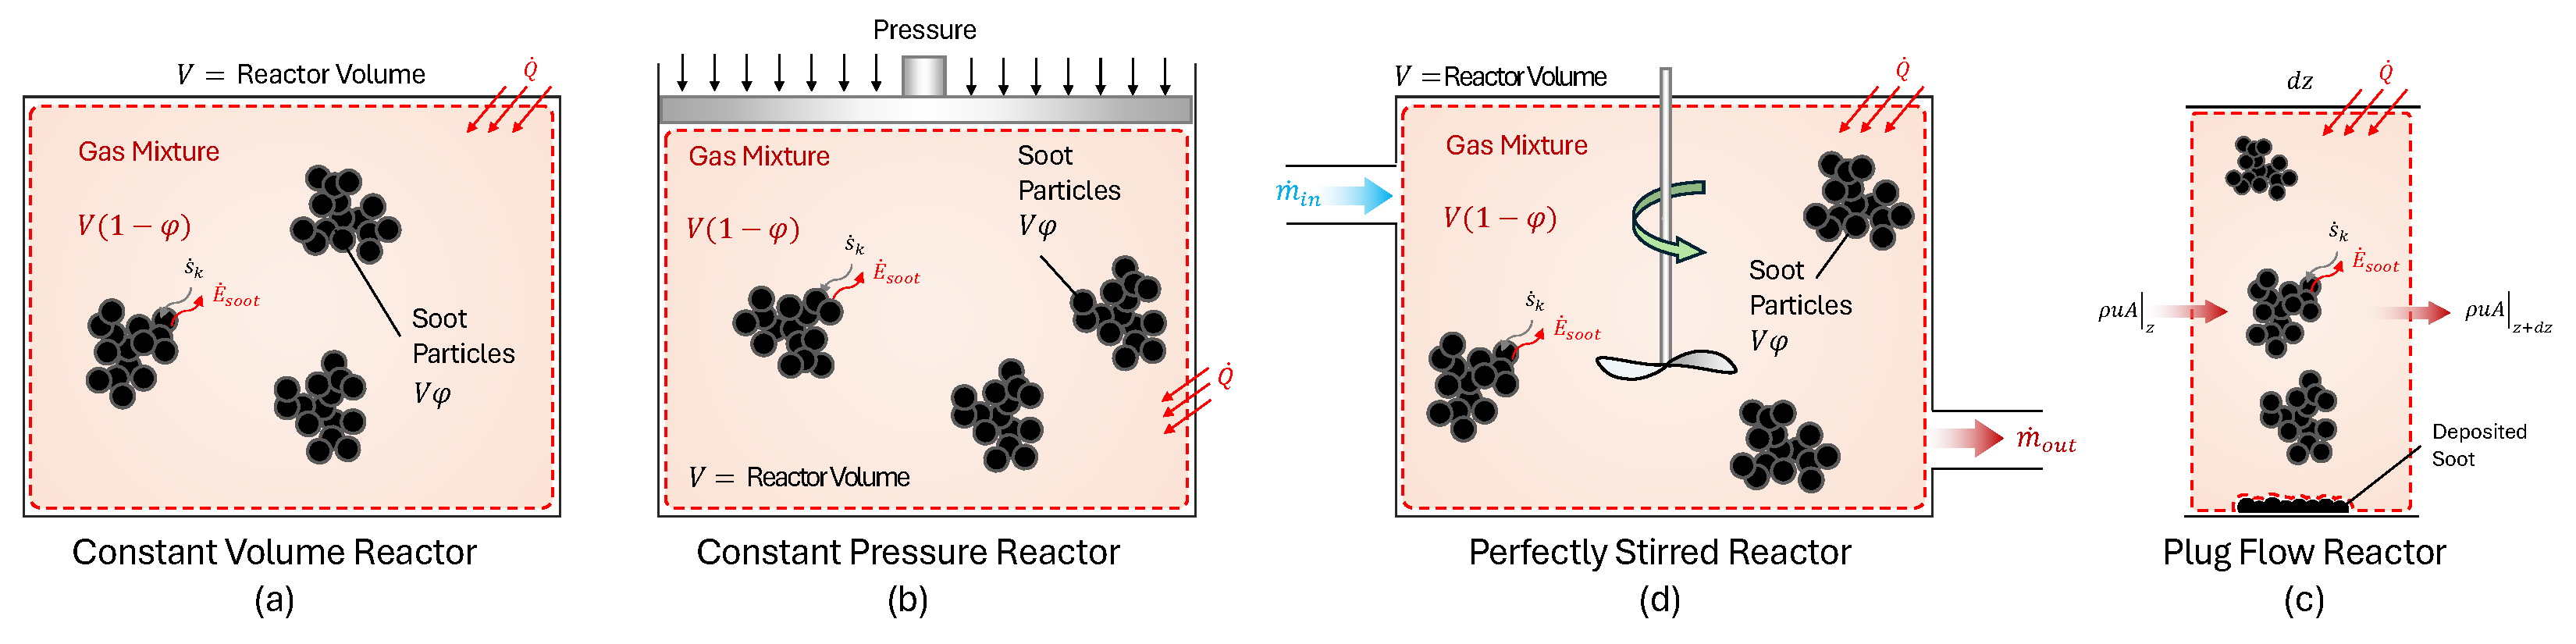
\includegraphics[width=1\textwidth]{Figures/Theory/reactors.pdf}
	\caption{The schematics of constant volume reactor (a), constant pressure reactor (b) perfectly stirred reactor (c), and plug flow reactor (d).}
	\label{fig:reactors} 
\end{figure}


\subsubsection{Constant Volume Reactor (CVR)}
\label{sec:cvr}
As shown in Figure~\ref{fig:reactors}a, CVR represents a closed system constant volume where chemical reactions converts part of the gas mixture to soot particles. The mass balance equation is written as:

\begin{equation}
	\frac{d}{dt}(m) = (1-\varphi)V \sum_i \dot s_i W_i,
	\label{eqn:contconstuv}
\end{equation} 

\noindent where $m$ is the mass of the gas mixture. The rate of change of $m$ is equal to the rate of production of soot mass.
Similarly, the species equation for species $k$ is expressed as:

\begin{equation}
	\frac{dY_k}{dt}
	=
	\frac{1}{\rho}
	\left(
		{\dot{\omega}}_k
		+
		{\dot{s}}_k
	\right)W_k
	-\frac{1}{\rho}Y_k\sum_{i}{{\dot{s}}_i W_i}
	\label{eqn:speciesconstuv}.
\end{equation}

The transport equation for a generic soot variable, $\psi$, can be written as:
\begin{equation}
	\frac{d \psi}{d t}= S_{\psi} - \frac{\psi}{\rho} \sum_i \dot{s}_i W_i
	\label{eqn:sootconstuv}.
\end{equation}

The second term on RHS of Equations~\eqref{eqn:speciesconstuv} and~\eqref{eqn:sootconstuv} denotes the change in $Y_k$ and $\psi$, respectively, due to the removal or addition of gas mass by soot-related processes.
The energy conservation for the gas mixture is written in terms of the rate of change of temperature. An external heat source of $\mathrm{\dot{Q}}$ is considered to account for possible heat loss/gain of the reactor.
\begin{equation}
	\begin{split}
		\frac{d T}{d t}=
		\frac{1}{\rho c_v+\rho_{soot}f_v c_{soot}}
		\left[
			-\sum_k e_k
				\left(
					\dot{\omega}_k+\dot{s}_k
				\right) W_k
		\right. \\
		\left.
			+e_{soot}\sum_k \dot{s}_k W_k
			+\frac{\dot{Q}}{V(1-\varphi)}
		\right],
	\end{split}
	\label{eqn:energyconstuv}
\end{equation}

\noindent where $\rho_{soot}f_v c_{soot}$ and $e_{soot}\sum_k \dot{s}_k W_k$ represent the formation and sensible energy of soot, respectively. We investigated the effect of considering soot formation and sensible energy on gas and soot properties by simulating the pyrolysis of 30\%~$\mathrm{CH_4}$-Ar with and without considering the above mentioned term. As shown in Figure~\ref{fig:sseeffect}a, neglecting soot sensible energy results in the overprediction of temperature by nearly 150 K and mobility diameter by a factor of 3 during the 80 ms of the simulation. The overprediction of temperature changes gas chemistry, leading to a noticeable decrease in the residual methane and benzene (Figure~\ref{fig:sseeffect}b).




\subsubsection{Constant Pressure Reactor (CPR)}

As show in Figure~\ref{fig:reactors}b, CPR is a closed system similar to CVR, but the pressure stays constant throughout the process, which means the boundaries of the system can move, changing its volume. The equations of mass, species, and soot variables in CPR are the same as those in CVR, but the energy equation is written based on enthalpy, $h$, instead of internal energy $e$, as:

\begin{equation}
	\begin{split}
		\frac{d T}{d t}=
		\frac{1}{\rho c_p+\rho_{soot}f_v c_{soot}}
		\left[
		-\sum_k h_k
		\left(
		\dot{\omega}_k+\dot{s}_k
		\right) W_k \right. \\
		\left.
		+h_{soot}\sum_k \dot{s}_k W_k
		+\frac{\dot{Q}}{V(1-\varphi)}
		\right]
		\label{eqn:energypressure}.
	\end{split}
\end{equation}

\subsubsection{Perfectly Stirred Reactor (PSR)}
In this reactor, gas enters with a mass flow rate, composition, and temperature of $\dot{m}_{in}$, $Y_{in}$, and $T_{in}$, respectively, and homogeneously reacts with the mixture inside the reactor. The reacting gas reaches a spatially uniform temperature and composition described by $T$, and $Y$. It is assumed that temperature, composition and soot properties of the outflow are the same as the mixture inside reactor. Without soot formation, the inlet and outlet mass flow rates are equal (i.e. ${\dot{m}_{in}}={\dot{m}_{out}}$), but when soot is formed, ${\dot{m}_{out}}$ is slightly less than ${\dot{m}_{in}}$. The nominal residence time of PSR is calculated as:

\begin{equation}
	\tau_{psr} = \frac{\rho V}{\dot{m}_{in}}
	\label{eqn:taupsr}.
\end{equation} 

The conservation of mass of PSR can be written by considering the mass flux of in- and outflow, and the removal of mass due to soot formation as:

\begin{equation}
	\frac{d m}{d t}
	=
	\dot{m}_{in} - \dot{m}_{out} 
	+ V(1 - \varphi)\sum_i \dot{s}_i W_i 
	\label{eqn:contpsr}.
\end{equation}

Gas composition is obtained by solving the species transport equations as:

\begin{equation}
	\frac{d Y_k}{d t}
	=
	\frac{{\dot{m}}_{in}}{\rho V
	\left(1-\varphi\right)}
	\left(Y_{k,in}-Y_k \right)+
	\frac{1}{\rho}\left[\left(\dot{\omega}_k+\dot{s}_k\right) W_k-Y_k \sum_i \dot{s}_i W_i\right]
	\label{eqn:speciespsr}.
\end{equation}

The soot transport equations can also be expressed as:
\begin{equation}
	\frac{d\psi}{dt}
	=
	\frac{{\dot{m}}_{in}}{\rho V
		\left(1-\varphi\right)}
	\left(\psi_{in}-\psi\right)
	+
	S_{\psi}
	-\frac{1}{\rho}\psi\sum_{i}{{\dot{s}}_i W_i}
	\label{eqn:sootpsr}.
\end{equation}

The energy equation for this reactor is written as:
\begin{equation}
	\begin{split}
		\frac{dT}{dt}
		=
		\frac{1}
		{
			\rho c_p+\rho_{soot}c_{p,soot}f_v
		}
		\left[
		\frac{{\dot{m}}_{in}}{V(1 - \varphi)}
		\left(h_{in}-h\right)
		-
		\frac{{\dot{m}}_{in}}{V (1 - \varphi)}\sum_{k}\left(Y_{k,in}-Y_k\right)h_k
		\right.\\
		\left.	
		-
		\sum_{k}{
			\left(
			{\dot{\omega}}_k
			+
			{\dot{s}}_k
			\right) W_k h_k}
		+\sum_{i}{{\dot{s}}_i W_i} h_{soot}+\frac{\dot{Q}}{V(1 - \varphi)}
		\right].
	\end{split}
		\label{eqn:energypsr}
\end{equation}



\subsubsection{Plug Flow Reactor (PFR)}
\label{sec:pfr}
PFR is an ideal representation of a channel or duct where the temperature, composition, and soot properties of a steady-state one-dimensional flow evolve along the reactor. There is no spatial gradient over cross-section due to strong mixing. The diffusion along reactor is negligible.
%\begin{figure}[!htbp]
%	\centering
%	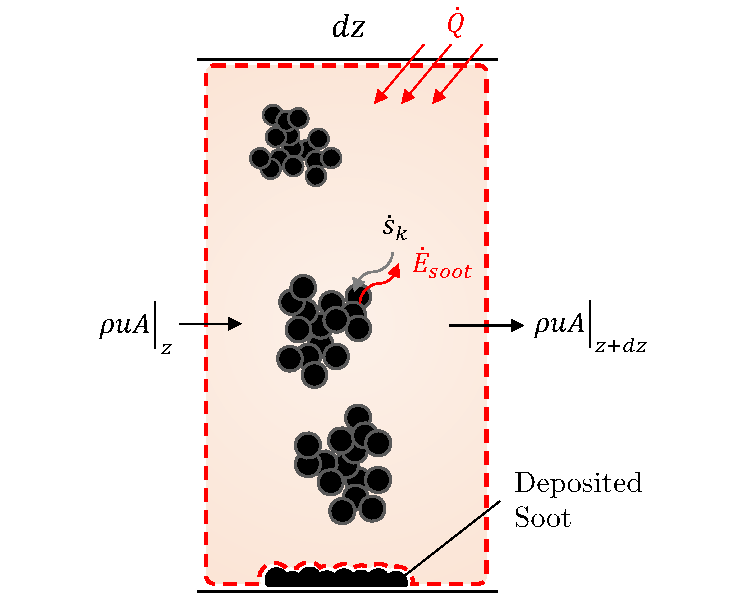
\includegraphics[height=50mm, ]{Figures/Theory/PFR.pdf}
%	\caption{The schematics of control volume for a differential element along PFR that includes the gas mixture and excludes the soot particles considering wall heat transfer. The model considers mass and energy are transfer between gas and soot as well as wall deposition along the reactor.}
%	\label{fig:pfrcv}
%\end{figure}


The continuity equation for PFR is written as:
\begin{equation}
	\frac{d\dot{m}}{dz} =(1-\varphi)A \sum_i \dot s_i W_i
	\label{eqn:contpfr}.
\end{equation}

The momentum equation can also be established as:
\begin{equation}
	u (1-f_v) \sum_i \dot s_i W_i + \rho u (1-\varphi) \frac{du}{dz}
	=-\frac{d}{dz}(p(1-\varphi))-\frac{\tau_{w}}{R_H} 
	\label{eqn:momenpfr},
\end{equation}
 \noindent where $\tau_w$, and $R_H$ is the wall shear stress and hydraulic radius of the reactor. $\tau_w$ can be determined from the friction factor, $f$, as:
\begin{equation}
	\tau_w = \frac{1}{2}\rho u^2 f, 
	\label{eqn:wallshearpfr}
\end{equation}

\noindent where $f$ can be calculated with a good accuracy for the entire range of Reynolds number, Re, from laminar to turbulent flow using the explicit formula given by \citet{haaland1983simple}:

\begin{equation}
	\frac{1}{f^{1/2}} = -1.8 \mathrm{log}
	\left(
		\frac{6.9}{Re}+
		\left[ \frac{\epsilon/D_H}{3.7} \right]^{1.11}
	\right)
	\label{eqn:fpfr},
\end{equation}
\noindent where $\epsilon$, and ${D_H}$ are the wall roughness and the hydraulic radius of the reactor. The species equation can be expressed as:
\begin{equation}
	\frac{d Y_k}{d z}=\frac{1}{\rho u}\left[\left(\dot{\omega}_k+\dot{s}_k\right) W_k-Y_k \sum_i \dot{s}_i W_i\right]
	\label{eqn:speciespfr}.
\end{equation}

 The soot transport equations can also be written as:
\begin{equation}
	\frac{d \psi}{d z}=
	\frac{S_{\psi}}{u}
	-\frac{\psi}{\rho u}\sum_i \dot{s}_i W_i
	-\frac{4}{D_H}\frac{k^i_{dep}\psi}{u},
	\label{eqn:sootpfr}
\end{equation}
\noindent where $k^i_{dep}$ is the deposition velocity of soot particles of section $i$, which is calculated as:

\begin{equation}
	k_{dep}=
	\frac{Sh\cdot D^i}{D_H},
	\label{eqn:kdep}
\end{equation}

\noindent where $Sh=3.66$ for laminar flows, and it calculated using the Berger and Hau correlation~\citep{berger1977mass} for the turbulent flow as:

\begin{equation}
	Sh=
	0.0165Re^{0.86} Sc^{1/3}
	\label{eqn:shdep}.
\end{equation}

The energy equation can be expressed as:
\begin{equation}
	\begin{split}
		\frac{d T}{d z}=
		\frac{1}{\rho u c_p+\rho_{soot} u f_v 	c_{p,soot}}
		\left[
			-\sum_k h_k
			\left(
			\dot{\omega}_k+\dot{s}_k
			\right) W_k
		\right. \\
		\left.
			+h_{soot}\sum_k \dot{s}_k W_k
			+q^{\prime \prime}\frac{P_c}{A}
		\right],
	\end{split}
	\label{eqn:energypfr}
\end{equation}
\noindent where $q^{\prime \prime}$ is the wall heat flux of the reactor.



\section{Particle dynamics}
\label{sec:particledynamics}
Population balance models rely on the Eulerian description of particles where average properties of particle population such as number density, mass or surface area are treated as continuous quantities and tracked by solving scalar transport equations. Here, we use two particle dynamics models: a monodisperse population balance model (MPBM), which tracks four variables and results in four transport equations, and a fixed sectional population balance model (SPBM), which tracks three variables per section. In the SPBM approach, the total number of transport equations equals the number of tracked variables multiplied by the number of sections. 

Having the total number concentration of agglomerates and primary particles and total carbon content of soot enables the model to describe evolving fractal-like morphology and surface area of soot agglomerates, which is essential to compute their collision frequency~\citep{mulholland1988cluster} as well as oxidation and surface growth rates~\citep{kelesidis2019estimating}. Tracking hydrogen content of soot allows capturing the soot composition, thereby its maturity~\citep{kholghy2016core}, and surface reactivity~\citep{blanquart2009analyzing}.

The common features of the implemented particle dynamics models include the composition (H/C), diffusion coefficient, and morphology of soot particles, all of which are calculated in the same manner for MPBM and for each section in SPBM. Soot morphology is reviewed in Section~\ref{sec:sootmorphology}, and the calculation of the diffusion coefficient is provided in Section~\ref{sec:diffcoef} of the supplementary material. 

However, the particle dynamics models differ in terms of calculating the coagulation partial source term, $I_{coag}$, and processing the contributions from inception, surface growth, oxidation, and coagulation, $I_{\varphi}$, to generate the source terms $S_{\varphi}$ that are incorporated into the transport equations.


%The common features of implemented particle dynamics models include the composition (H/C), diffusion coefficient, and morphology of soot particles, which are calculated in the same manner for MPBM and each section in SPBM. The soot morphology is reviewed in Section~\ref{sec:sootmorphology}, and the calculation of diffusion coefficient can be found in Section~\ref{sec:diffcoef} of the supplementary material. However, particle dynamics models differ in terms of the calculation of coagulation partial source term, $I_{coag}$, and processing of the contributions from inception, surface growth, oxidation, and coagulation, $I_{\varphi}$, to generate the source terms, $S_{\varphi}$, that are incorporated into the transport equations.

\subsection{Soot morphology}
\label{sec:sootmorphology}

The evolving fractal-like structure of agglomerates is quantified by their mobility diameter normalized by primary particle diameter, $d_m/d_p$, and gyration diameter, $d_m/d_g$, that can be described with power-laws derived from mesoscale simulations.
Incipient soot is initially a sphere formed of PAHs with constant density that grows in size by surface reactions and forms agglomerates by coagulation. The collision frequency of particles depends on their evolving fractal-like structure~\citep{mulholland1988cluster}.
Mobility and gyration diameters are calculated using power-laws developed to describe the morphology of soot from premixed~\citep{abid2008evolution}, diffusion~\citep{yon2015simple} flames, and diesel engines~\citep{rissler2013effective}. Figure~\ref{fig:Morphology} shows a schematic of a soot agglomerate composed of 12 primary particles, with ${d_p}$, ${d_m}$, and ${d_g}$ annotated.
\begin{figure}[!htbp]
	\centering
	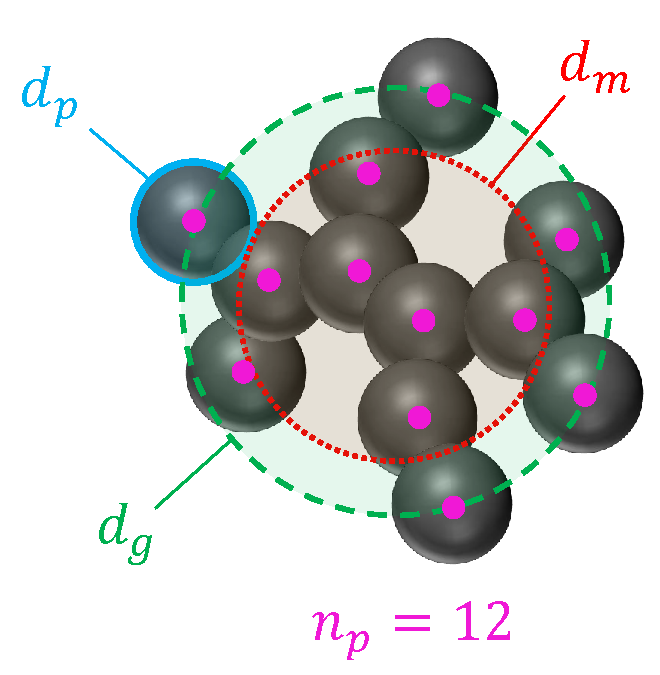
\includegraphics[height=60mm, ]{Figures/Theory/Morphology.pdf}
	\caption{The schematics of a soot agglomerates with 12 primary particles (${n_p=12}$). Primary particle, ${d_p}$, mobility, ${d_m}$, and gyration, ${d_g}$, diameters are shown.}
	\label{fig:Morphology}
\end{figure} 


${n^i_p}$ is the number of primary particles per agglomerate of ${i^{th}}$ section that can be obtained by dividing the number concentration of primary particles in ${i^{th}}$ section by that of agglomerates in that section as:

\begin{equation}
	n^i_p = \frac{N^i_{pri}}{N^i_{agg}}
	\label{eqn:n_p}.
\end{equation}

Primary particle diameter, ${d^i_p}$, is determined from total carbon content and number density of primary particles using:

\begin{equation}
	d^i_p = \left(\frac{6}{\pi} \frac{C^i_{tot}\cdot W_{carbon}}{\rho_{soot}} \frac{1}{N^i_{pri}\cdot Av} \right)^{1/3}.
	\label{eqn:d_p}
\end{equation}

The DEM-derived power-laws~\citep{Kelesidis2017} relate ${d^i_m}$ and ${d^i_g}$ to ${d^i_p}$ and ${n^i_p}$ as:

\begin{equation}
	d^i_{m} = d^i_p\cdot {n^i_p}^{0.45}
	\label{eqn:d_m},
\end{equation}

\begin{equation}
	d^i_g = 
	\left\{
	\begin{array}{lr}
		d^i_m/({n^i_p}^{-0.2}+0.4), & \text{if } n^i_p > 1.5\\
		d^i_m/1.29. & \text{if } n^i_p\leq 1.5
	\end{array}
	\right.
	\label{eqn:d_g}
\end{equation}

The collision diameter, ${d^i_c}$, is the maximum of ${d^i_{m}}$ and ${d^i_{g}}$:

\begin{equation}
	d^i_c = \mathrm{max}\left(d^i_m, d^i_g\right).
	\label{eqn:d_c}
\end{equation}

$A^i_{tot}$ (for each section) is defined as the total surface area of soot particles per unit mass of gas mixture obtained as:
\begin{equation}
	A^i_{tot} = N^i_{pri}\cdot Av\cdot \pi {d^i_p}^2
	\label{eqn:Atot}.
\end{equation}

Mass of each agglomerate, $m^i_{agg}$, is expressed as:
\begin{equation}
	m^i_{agg} = \frac{C^i_{tot}\cdot W_{carbon}}{N^i_{agg}\cdot Av}.
	\label{eqn:m_agg}
\end{equation}





\subsection{Sectional Population Balance Model (SPBM)}
A SPBM with the fixed pivot is used to describe particle dynamics~\citep{wu1988discrete}. The mass range of particles are divided into discrete sections each of which includes agglomerates of the same mass. Figure~\ref{fig:sectional} illustrates the interaction between the gas phase and mass sections, as well as the mechanisms by which particles move between sections. Inception introduces new particles to the first section with the mass corresponding to the incipient particle. The particles of each section can migrate to upper sections by gaining mass via surface growth and coagulation, and return to lower sections when they lose mass through oxidation without breaking into smaller particles (i.e., fragmentation is not considered). Particles attach at point contact without coalescence. The mass of sections is determined by a geometric progression that has an initial equal to the mass of incipient soot particle, and a common ratio of SF, known as sectional spacing factor. The mass of each section is approximated by the carbon content of agglomerates in moles as:
\begin{equation}
	C^i_{agg} = \frac{n_{c,min}}{Av}\cdot SF^{(i-1)},
	\label{eqn:Caggsec}
\end{equation}
\noindent where $(i-1)$ represents the exponent of SF. The mass of hydrogen is ignored in the placement of agglomerates in the sections.
The total number density of agglomerates, $N^i_{agg}$ and primary particles, ${N^i_{pri}}$, and the hydrogen content, $H_{tot}$ are tracked for each section. The mass of each section is fixed, so $C_{tot}$ for each section can be easily calculated by knowing the number of agglomerates; that is, $C_{tot} = N^i_{agg} \cdot \mathrm{Av} \cdot C^i_{agg}$. Morphological parameters for each section are determined according to the equations provided in Section~\ref{sec:sootmorphology}.


\begin{figure}[!htbp]
	\centering
	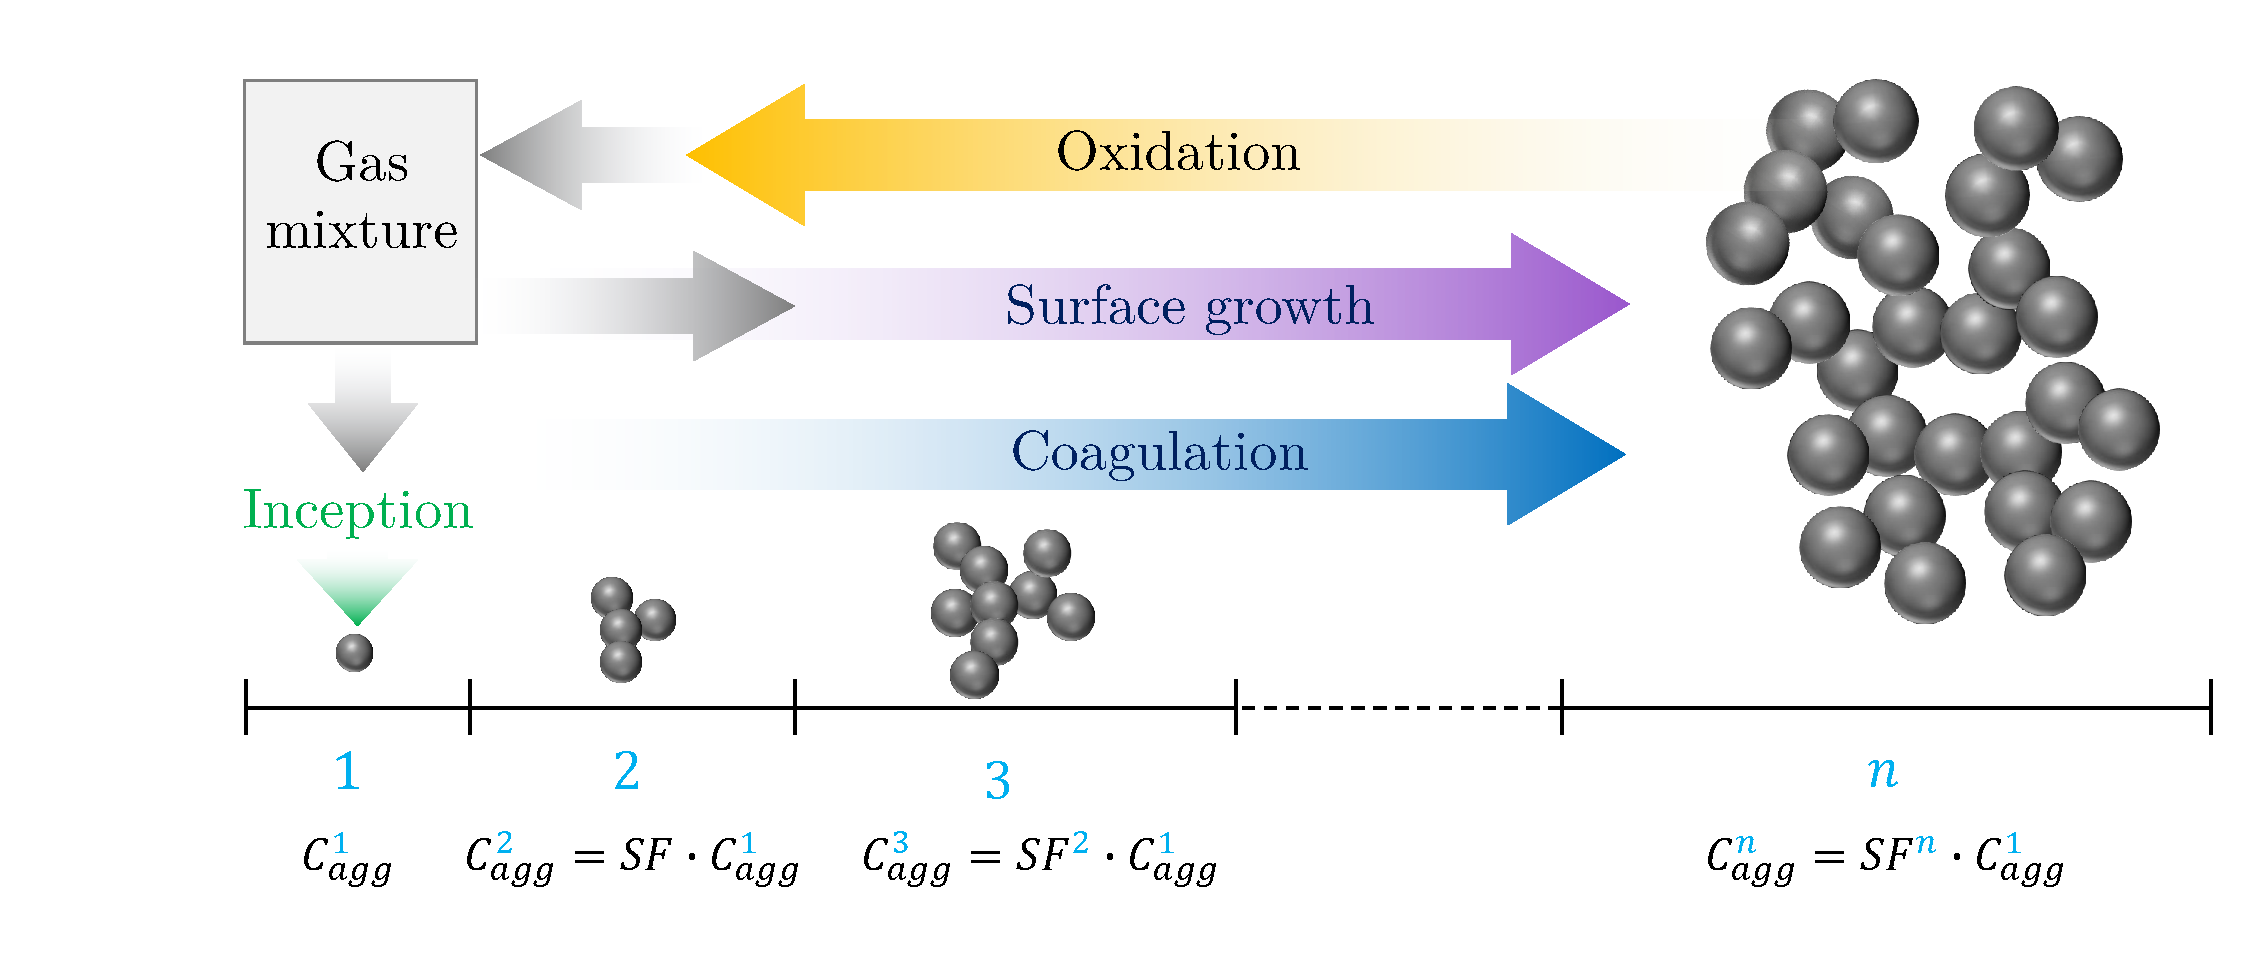
\includegraphics[height=40mm, ]{Figures/Theory/Sectional.pdf}
	\caption{The illustration of mass sections in SPBM that grow progressively by the scale factor of SF. Inception introduces new particles to the first section that propagate to the upper section via coagulation and surface growth and return to lower sections by oxidation. Carbon and hydrogen pass from gas to solid phase through inception and surface growth and goes back via oxidation.}
	\label{fig:sectional}
\end{figure}
 
New particles formed by coagulation are assigned to an upper section, with a total mass equal to the sum of the masses of the colliding particles. If the mass of resulting particle falls between two consecutive sections, the mass is distributed between them proportionally. In some cases, the mass of the newly formed particle may exceed the upper bound of the last section, causing it to fall outside the tracked mass range. This leads to potential mass loss, which is a known limitation of the fixed pivot sectional model~\citep{zhang2010detailed}. However, this issue can be mitigated by choosing an appropriate number of sections and a suitable spacing factor to ensure the uppermost sections remain unoccupied during the simulation. In the SPBM, the source terms of tracked soot variables (which appear in Equations~\ref{eqn:sootconstuv},~\ref{eqn:sootpsr},~and~\ref{eqn:sootpfr}) are split into four parts showing the contribution of inception, surface growth, oxidation and coagulation. The effect of HACA and PAH adsorption are combined (denoted by the subscript \textit{haca,ads}) because they are similar mass-gaining mechanisms. The source terms for section $i$ are given as:

\begin{equation}
	S^i_{N_{agg}} = 
	\left(S^i_{N_{agg}}\right)_{inc}
	+\left(S^i_{N_{agg}}\right)_{haca, ads}
	+\left(S^i_{N_{agg}}\right)_{ox}
	+\left(S^i_{N_{agg}}\right)_{coag}
	\label{eqn:S_Naggsect},
\end{equation}

\begin{equation}
	S^i_{N_{pri}} = 
	\left(S^i_{N_{pri}}\right)_{inc}
	+\left(S^i_{N_{pri}}\right)_{haca, ads}
	+\left(S^i_{N_{pri}}\right)_{ox}
	+\left(S^i_{N_{pri}}\right)_{coag}
	\label{eqn:S_Nprisect},
\end{equation}

\begin{equation}
	S^i_{H_{tot}} = 
	\left(S^i_{H_{tot}}\right)_{inc}
	+\left(S^i_{H_{tot}}\right)_{haca, ads}
	+\left(S^i_{H_{tot}}\right)_{ox}
	+\left(S^i_{H_{tot}}\right)_{coag}
	\label{eqn:S_Htotsect}.
\end{equation}

The calculation of coagulation source terms is based on the implementation of SPBM by \citet{veshkini2015understanding}, and it is presented in detail along with the other source terms in Section~\ref{sec:sectextra} of the supplementary material.


\subsection{Monodisperse Population Balance Model (MPBM)}
\label{sec:mpbm}
The MPBM used in this study is based on the monodisperse model presented in \citep{kholghy2021surface}, and it tracks $N_{pri}$, $N_{agg}$, $C_{tot}$ and $H_{tot}$. The coagulation model follows the same principles as the SPBM, but the calculations are greatly simplified due to the monodispersity assumption. This approach has been shown to achieve accuracy comparable to that of DEM and SPBM when applied with well-justified assumptions~\citep{Kelesidis2017Flame, kelesidis2019estimating}. The rate of decay of agglomerates is simply described as:

\begin{equation}
	I_{coag} = -\frac{1}{2}\zeta\beta N^2_{agg}
	\label{eqn:Icoag},
\end{equation}
where $\zeta$ is the collision efficiency of agglomerates calculated using Equation~\eqref{eqn:coageff}, and ${\beta}$ is the collision frequency of agglomerates for the free-molecular ($\mathrm{Kn>10}$) to continuum regimes (${Kn<0.1}$). The value of ${\beta}$ in the transition regime (${0.1<Kn<10}$) can be calculated from the harmonic mean of the continuum (${\beta_{cont}}$) and free-molecular (${\beta_{fm}}$) regime values. Additionally, an enhancement factor of \%82 is applied to take into account the effect of polydispersity~\citep{kelesidis2021self} as:
\begin{equation}
	\beta = 1.82\frac{\beta_{fm}\cdot\beta_{cont}}{\beta_{fm}+\beta_{cont}}
	\label{eqn:betahmmono},
\end{equation}
\begin{equation}
	\beta_{fm} = 4\sqrt{\frac{\pi k_B T}{m_{agg}}} d^2_c
	\label{eqn:betafmmono},
\end{equation}
\begin{equation}
	\beta_{cont} = 8\pi d_m D,
	\label{eqn:betacontmono}
\end{equation}
\noindent where $d_c$, $D$, and $m_{agg}$ are calculated using Equations~\eqref{eqn:d_c},~\eqref{eqn:diff},~and~\eqref{eqn:m_agg}, respectively.
Alternatively, $\mathrm{\beta}$ can be obtained using Fuchs interpolation~\citep{fuchs1965mechanics} as:

\begin{equation}
	\beta = \beta_{cont}
	\left(
		\frac{d_c}{d_c+2\sqrt{2}\delta} +
		\frac{8D}{\sqrt{2}c d_c}
	\right)^{-1},
	\label{eqn:betafuchsmono}
\end{equation}
\noindent where $c$ (mean velocity of particles) and $\delta$ (mean stop distance of particles) are calculated using Equations~\eqref{eqn:meanvel}~and~\eqref{eqn:meandist}. The source terms of tracked variables combines the effect of the inception, surface growth, oxidation and coagulation.

\begin{equation}
	S_{N_{agg}} = \frac{I_{N,inc}}{n_{c,min}}+I_{coag},
	\label{eqn:S_N_agg}
\end{equation}
\begin{equation}
	S_{N_{pri}} = \frac{I_{N,inc}}{n_{c,min}},
	\label{eqn:S_N_pri}
\end{equation}
\begin{equation}
	S_{C_{tot}} = I_{C_{tot},inc}+I_{C_{tot},haca}+I_{C_{tot},ads} - I_{C_{tot},ox},
	\label{eqn:S_C_tot}
\end{equation}
\begin{equation}
	S_{H_{tot}} = I_{H_{tot},inc}+I_{H_{tot},haca}+I_{H_{tot},ads} - I_{H_{tot},ox}.
	\label{eqn:S_H_tot}
\end{equation}


\section{PAH growth models}
\label{sec:pahgrowmodel}
Four different PAH growth models are implemented in Omnisoot to describe the conversion of PAHs into incipient particles and their adsorption onto existing agglomerates. In other words, these models explain the calculation of $I_{\phi, inc}$ and $I_{\phi, ads}$. The implemented models are: Irreversible Dimerization~\cite{frenklach1991detailed}, Reactive Dimerization~\citep{kholghy2018reactive}, Dimer Coalescence~\citep{blanquart2009joint}, and E-Bridge Modified~\citep{frenklach2020mechanism}. All models are based on PAH collision, as supported by ample evidence in the literature~\citep{zhao2003measurement, abid2009quantitative, happold2009soot}, but they differ in terms of reversibility, temperature dependence, and the number of steps involved. The formulation and implementation details of the first three models are provided in Sections~\ref{sec:irrevdim}-\ref{sec:dimcoal} of the supplementary material, while only E-Bridge Modified model is discussed here for brevity.

The collision frequency of gaseous species, including PAH molecules and polymers, depends on their mass and diameter and is calculated as:

\begin{equation}
	\beta_{dim_{jk}}=
	2.2 \cdot d^2_{r} \sqrt{\frac{8 \pi k_B T}{m_{r}}},
	\label{eqn:betadim}
\end{equation}

\noindent where 2.2 is the vdW enhancement factor~\citep{kholghy2018reactive}. ${d_{r}}$ and ${m_{r}}$ are reduced diameter and mass for two PAH molecules/dimers, respectively, calculated as:

\begin{equation}
	d_{r}=
	\frac{d_{{PAH}_k}\cdot d_{{PAH}_j}}{d_{{PAH}_k}+d_{{PAH}_k}},
	\label{eqn:drPAH}
\end{equation}

\begin{equation}
	m_{r}=
		\frac{m_{{PAH}_k}\cdot m_{{PAH}_j}}{m_{{PAH}_j}+ m_{\mathrm{PAH}_k}},
	\label{eqn:mrPAH}
\end{equation}

\noindent where $m_{PAH_j}$ and $d_{PAH_j}$ are the mass and equivalent diameter of the ${j}^{th}$ PAH molecule, respectively, and are obtained as:

\begin{equation}
	m_{PAH_j}=
	\frac{W_{{PAH}_j}}{Av},
	\label{eqn:mPAH}
\end{equation}

\begin{equation}
	d_{PAH_j}=
	\left(
		\frac{6\cdot m_{{PAH}_j}}{\pi\cdot\rho_{{PAH}_j}}
	\right)^{1/3},
	\label{eqn:dPAH}
\end{equation}

\noindent where $\rho_{PAH_j}$ is the equivalent density of PAH estimated using the relation proposed by \citet{johansson2016formation} as:

\begin{equation}
	\rho_{PAH_j}= 
	171943.5197
	\frac{W_{carbon}\cdot n_{C,{PAH}_j}+W_{hydrogen}\cdot n_{H,{PAH}_j}}
	{n_{C,{PAH}_j}+n_{H,\mathrm{PAH}_j}},
	\label{eqn:rhoPAH}
\end{equation}

\noindent where ${n_{C,{PAH}_j}}$ and ${n_{H,{PAH}_j}}$ denote the number of carbon and hydrogen atoms in the $j^{th}$ PAH molecule, respectively. The collision frequency of $\mathrm{PAH}_j$ and soot agglomerates in each section can be determined for the entire regime by harmonic mean of the collision frequencies in the free-molecular and continuum regimes as:

\begin{equation}
	\beta^i_{ads_j}=
	\frac{\beta^i_{fm, ads}\cdot \beta^i_{cont, ads}}
	{\beta^i_{fm, ads}+\beta^i_{cont, ads}},
	\label{eqn:betahmads}
\end{equation}

\begin{equation}
	\beta^i_{fm, ads_j}=
	2.2 
	\sqrt{
		\frac{\pi k_B T}{2}\left(\frac{1}{m^i_{agg}}+\frac{1}{m_{PAH_j}}\right)
	}
	\left(d^i_g+d_{PAH}\right)^2,
	\label{eqn:betafmads}
\end{equation}

\begin{equation}
	\beta^i_{cont, ads_j}=
		\frac{2 k_B T}{3 \mu}
		\left[
			\frac{C^i\left(d_m\right)}{d^i_g}+
			\frac{C^i\left(d_{PAH_j}\right)}{d_{PAH_j}}
		\right]
		\left(d_g+d_{PAH_j}\right),
	\label{eqn:betacontads}
\end{equation}
where $C^i$ is the Cunningham correction factor calculated using Equation~\eqref{eqn:cun}.

\subsection{E-Bridge Modified}
\label{sec:ebrimod}
The E-Bridge model was originally proposed by \citet{frenklach2020mechanism} to describe soot inception using a HACA-like scheme that starts with the dehydrogenation of PAH monomers, often pyrene, which forms the monomer radicals and continues with the sequential addition of the radicals to PAHs that form dimers, trimers and larger polymers until the PAH structure reaches the mass threshold and the clustering process becomes irreversible~\citep{frenklach2020mechanism}. Here, a modified version of this model, called E-Bridge Modified, is used where dimers are considered as incipient soot, and monomer radical are adsorbed on soot agglomerates. This PAH growth model is described using the following set of pathways:

\reaction[reac:dehyd_ebri]{
	PAH_j + H <-->[$k_{f,d_{j}}$][$k_{r,d_{j}}$] $\mathrm{\dot{PAH}}_j$ + H
}

\reaction[reac:hyd_ebri]{
	$\mathrm{\dot{PAH}}_j$ + H ->[$k_{f,h_{j}}$] PAH_$j$ 
}

\reaction[reac:ebri]{
	$\mathrm{\dot{PAH}}_j$ + PAH_j ->[$k_{inc_j}$] Dimer_{$j$}
}
\reaction[reac:ads_ebri]{
	$\mathrm{\dot{PAH}}_j$ + Soot ->[$k_{ads_j}$] Soot-PAH_{$j$}
}

The rate constants of Reactions~\eqref{reac:dehyd_ebri}~and~\eqref{reac:hyd_ebri} are listed in Table~\ref{tab:Ebridge} while those of dimer production and adsorption are calculated based on Equations~\eqref{eqn:betadim}~and~\eqref{eqn:betahmads}, respectively. For both steps, it is assumed that all collisions are successful i.e., 100\% collision efficiency for radical-monomer and radical-soot.

\begin{equation}
	k_{inc_j}=
	\beta_{jj,PAH}\cdot Av
	\label{eqn:kdim_ebri},
\end{equation}

\begin{equation}
	k^i_{ads_{j}}=
	\beta^i_{ads_j}\cdot Av
	\label{eqn:kads_ebir},
\end{equation}

\renewcommand{\arraystretch}{1.5}
\begin{table}
	\caption{Rate coefficients for the monomer de-/hydrogenation reaction of E-bridge formation in Arrhenius form $\mathrm{k=AT^n\cdot e^{-E/RT}}$~\citep{frenklach2020mechanism}.}
	\label{tab:Ebridge}
	\centering
	\begin{tabular}{l l l l l}
		\hline
		Reaction & \hspace{0.1cm} & A~$\mathrm{\left[{m^3}/{mol\cdot s} \right]}$ & n & $\mathrm{{E}/{R} [K]}$  \\
		\hline
		\eqref{reac:dehyd_ebri} & f & $98\times$ $\mathrm{n_{C, PAH_j}}$ & 1.8 & 7563.519 \\
		  & r & $1.6\times 10^{-2}$ & 2.63 & 2145.346\\
		\eqref{reac:hyd_ebri} & f & $4.8658\times10^7
		$ & 0.13 & 0.0\\
		\hline
	\end{tabular}
\end{table}

\noindent where $\beta_{jj,PAH}$, and $\beta^i_{ads_j}$ are calculated using Equations~\eqref{eqn:betadim}~and~\eqref{eqn:betahmads}, respectively. The rate of dimer formation and adsorption is calculated as:

\begin{equation}
	w_{dim_j} = k_{inc_{j}} [\mathrm{PAH}_j] [\mathrm{\dot{PAH}}_j],
	\label{eqn:wdim_ebri}
\end{equation}

\begin{equation}
	w^i_{ads_j} = k^i_{ads_{j}} [\mathrm{soot}^i] [\mathrm{\dot{PAH}}_j].
\end{equation}

The calculation of rate of inception and PAH adsorption from $\mathrm{PAH}_j$ requires the concentration of $\mathrm{\dot{PAH}}_j$, which can be determined by applying the steady-state assumption for $\mathrm{\dot{PAH}_j}$, i.e., $d[\mathrm{\dot{PAH}}_j]/dt=0$, resulting in a quadratic equation as:

%\begin{equation*}
%	\frac{d[\mathrm{\dot{PAH}_j}]}{dt} = 0
%\end{equation*}

%\begin{equation*}
%\begin{aligned}
%	&&k_{f,d_j}[\mathrm{PAH_j}][\mathrm{H}]
%	-k_{r,d_j}[\mathrm{\dot{PAH}_j}][\mathrm{H_2}]
%	-k_{f,h_j}[\mathrm{\dot{PAH}_j}][\mathrm{H}]
%	-k_{inc_j}[\mathrm{\dot{PAH}_j}]^2 &\\
%	&&-\sum_{i=1}^{n_{sec}}k^i_{ads_j}[\mathrm{\dot{PAH}_j}][\mathrm{Soot}]^i
%	&= 0
%\end{aligned}
%\end{equation*}

%The above equations can be rearranged as a quadratic equation similar to the dimer coalescence.

\begin{equation}
	a_{inc_j}[\mathrm{\dot{PAH}_j}]^2+
	b_{ads_j}[\mathrm{\dot{PAH}_j}] + c_j = 0,
\end{equation}
\begin{equation}
	a_{inc_j}=k_{inc_j}
\end{equation}
\begin{equation}
	b_{ads_j}=k_{r,d_j}[\mathrm{H_2}]+k_{f,h_j}[\mathrm{H}]+\sum_{i=1}^{n_{sec}}k^i_{ads_j}[\mathrm{Soot}]^i
\end{equation}
\begin{equation}
	c_{inc_j}=k_{f,d_j}[\mathrm{PAH_j}][\mathrm{H}]
\end{equation}

Solving the quadratic equation for each PAH gives the concentration of $\mathrm{\mathrm{\dot{PAH}}}_j$ as:
\begin{equation}
	[\mathrm{\mathrm{\dot{PAH}}_j}]=
	\left\{
	\begin{aligned}
		&\frac{-b_{ads_j}+\sqrt{\Delta_j}}{2a_{inc_j}},
		&&
		\text{if } \Delta_j \ge 0
		\\
		& 0 
		&&
		\text{if } \Delta_j < 0
	\end{aligned}
	\right.
	\label{eqn:rad_ebri}
\end{equation}
\begin{equation}
	\Delta_j = b_{ads_j}^2-4a_{inc_j}c_{j}
	\label{eqn:delta_ebri}
\end{equation}

The contribution of inception and adsorption to the partial source terms for E-Bridge formation can be written as:

\begin{equation}
	I_{N,{inc}} = \frac{1}{\rho}
	\sum_{j=1}^{n_{PAH}}
	2\omega_{inc_{j}}
	n_{PAH_j,C}
	\label{eqn:IN_inc_ebri},
\end{equation}

\begin{equation}
	I_{C_{tot},{inc}} = \frac{1}{\rho}
	\sum_{j=1}^{n_{PAH}}
	2\omega_{inc_{j}} 
	n_{PAH_j,C}
	\label{eqn:ICtot_inc_ebri},
\end{equation}

\begin{equation}
	I_{H_{tot},{inc}} = \frac{1}{\rho}
	\sum_{j=1}^{n_{PAH}}
	2\omega_{inc_{j}} 
	\left(
	n_{PAH_j,H}-2
	\right)
	\label{eqn:IHtot_inc_ebri},
\end{equation}

\begin{equation}
	I^i_{C_{tot},ads} =
	\frac{1}{\rho}
	\sum_{i=1}^{n_{PAH}}
	\omega^i_{ads_j}
	n_{C,PAH_j}
	\label{eqn:ICtotads_ebri},
\end{equation}

\begin{equation}
	I^i_{C_{tot},ads} =
	\frac{1}{\rho}
	\sum_{i=1}^{n_{PAH}}
	\omega^i_{ads_j}
	\left(n_{H,PAH_j}-2\right)
	\label{eqn:IHtotads_ebri}.
\end{equation}

The rate of removal of each PAH involved in soot inception and PAH adsorption, and release of $\mathrm{H_2}$ to the gas mixture can be expressed as:

\begin{equation}
	\left(
	\frac{d\left[{\mathrm{PAH_j}}\right]}{dt}
	\right)_{inc}
	= 
	-2\sum_{k=1}^{n_{PAH}}w_{inc_{j}},
\end{equation}

\begin{equation}
	\left(
	\frac{d\left[{\mathrm{PAH_j}}\right]}{dt}
	\right)_{inc}
	= 
	-\sum_{i=1}^{n_{sec}}w^i_{ads_j},
	\label{eqn:PAHscrub_ebri_ads}
\end{equation}

\begin{equation}
	\left(
	\frac{d\left[{\mathrm{H_2}}\right]}{dt}
	\right)_{inc}
	= 
	\sum_{i=1}^{n_{sec}}w^i_{ads_j}.
	\label{eqn:H2scrub_ebri}
\end{equation}

\section{Surface reactions model}
\label{sec:surfreacmodel}
The heterogeneous surface reactions are described by HACA. The soot growth in HACA scheme is based on a sequential process similar to PAH growth. The hydrogenated arm-chair sites ($\mathrm{C_{soot}-H}$) on the edge of aromatic rings are dehydrogenated by H abstraction forming $\mathrm{C_{soot\mbox{\textdegree}}}$ that bonds with $\mathrm{C_2H_2}$ resulting in an additional aromatic ring with hydrogenated site. These sites can also be attacked by $\mathrm{O_2}$ or $\mathrm{OH}$ leading to removal of carbon from soot particles by oxidation. The elementary reactions that describe this sequential process are listed in Table~\ref{tab:HACA}.
The rate of mass growth by HACA is obtained from the reaction of $\mathrm{C_2H_2}$ with dehydrogenated sites as:

\begin{equation}
	\omega^i_{gr} = \alpha^i k_{f4} [\mathrm{C_2H_2}][\mathrm{C_{soot\mbox{\textdegree}}}]
	\label{eqn:hacaRate},
\end{equation}

\noindent  where ${k_{f4}}$ denotes the forward rate of Reaction~\eqref{reac:haca4} in Table~\ref{tab:HACA}, and $\mathrm{[C^i_{soot\mbox{\textdegree}}]}$ is obtained by multiplying the surface density of dehydrogenated sites, $\mathrm{\chi_{soot\mbox{\textdegree}}}$ with total surface area of soot (per unit of mass of gas mixture) as:

\begin{equation}
	[\mathrm{C^i_{soot\mbox{\textdegree}}}] = \frac{\rho}{Av}A^i_{tot}\cdot\chi_{soot\mbox{\textdegree}}
	\label{eqn:csoot0},
\end{equation}

\noindent where $\mathrm{\chi_{soot\mbox{\textdegree}}}$ is the surface density of dehydrogenated sites, and is calculated by assuming the steady-state for $\mathrm{[C_{soot\mbox{\textdegree}}]}$ in the system of reactions in Table~\ref{tab:HACA} as:
\begin{equation}
	\chi_{soot{\mbox{\textdegree}}} = 
	\frac
	{k_{f1}[\mathrm{H}]+k_{f2}[\mathrm{OH}]}
	{k_{r1}[\mathrm{H_2}]+k_{r2}[\mathrm{H_2O}]+k_{f3}[\mathrm{H}]+k_{f4}[\mathrm{C_2H_2}]+k_{f5}[\mathrm{O_2}]} \chi_{soot-{H}},
	\label{eqn:chisoot0}
\end{equation}
\noindent where ${\chi_{soot-{H}}}$ is the surface density of hydrogenated sites estimated based on the assumption that soot ``surface is assumed to be composed of outwardlooking PAH edges with PAH molecular moieties assembled into turbostratic structures"~\citep{frenklach2019new}. Considering the layer spacing of 3.15$\mathrm{\AA}$ and 2 C–H bonds per benzene ring length, the surface density of hydrogenated sites, $\chi_{{soot}-H}$, is calculated to be $0.23\:\mathrm{site/\AA^2}=2.3\times10^{19}$ $ \mathrm{site/m^2}$, which gives the maximum theoretical limit of the reaction sites.

In Equation~\eqref{eqn:hacaRate}, $\alpha$ is the surface reactivity factor between 0 and 1 that represents the decline of reaction sites from the theoretical limit due to PAH layer orientation, particle aging, growth and maturity~\citep{haynes1982surface, harris1985chemical}, and it has been observed to depend on temperature-time-history~\cite{homann1985formation, dasch1985decay}. The value of $\alpha$ has been described using constant target-specific values as well as empirical equations based on particle size and flame temperature. A detailed review of these can be found in the chapter 4 of \citep{veshkini2015understanding}.  Here, the empirical equation proposed by \citet{appel2000kinetic} is used to calculate $\mathrm{\alpha}$:
\begin{equation}
	\alpha^i = \tanh 
	\left(
	\frac{12.56 - 0.00563\cdot T}
	{\mbox{log}_{10}
		\left( \frac{\rho_{soot}\cdot Av}{W_{carbon}} \frac{\pi}{6}{d^i_p}^3 \right) } -1.38+0.00068\cdot T
	\right)
	\label{eqn:alpha}.
\end{equation}

Alternatively, $\mathrm{\alpha}$ can be related to the H/C ratio of soot particles by assuming that all hydrogen atoms reside on the particle surface~\citep{blanquart2009joint} as:

\begin{equation}
	\alpha^i = \frac{H^i_{tot}}{C^i_{tot}}
	\label{eqn:alpha_htoc}.
\end{equation}

The contribution of HACA to growth source terms can be computed from HACA rates considering the number of carbon atoms in $\mathrm{C_2H_2}$ and number of arm-chair and zig-zag hydrogenated sites on soot particle~\cite{blanquart2009analyzing} using

\begin{equation}
	I^i_{C_{tot},gr} = 2\omega^i_{gr}/\rho
	\label{eqn:IiCtotgr},
\end{equation}
\begin{equation}
	I^i_{H_{tot},gr} = 0.25\omega^i_{gr}/\rho
	\label{eqn:IiHtotgr}.
\end{equation}

The rate of concentration change of $\mathrm{C_2H_2}$, and H radical due to HACA is written as:

\begin{equation}
	\left(\frac{d\left[{\mathrm{C_2H_2}}\right]}{dt}\right)_{gr} = -\sum_{i=1}^{n_{sec}}\omega^i_{gr},
	\label{eqn:C2H2rate_gr}
\end{equation}

\begin{equation}
	\left(\frac{d\left[{\mathrm{H}}\right]}{dt}\right)_{gr} = 1.75 \sum_{i=1}^{n_{sec}}\omega^i_{gr}.
	\label{eqn:Hrate_gr}
\end{equation}





\renewcommand{\arraystretch}{1.5}
\begin{table}
	\caption{Arrhenius rate coefficients of the various surface reactions in HACA~\citep{appel2000kinetic}, $\mathrm{k=AT^n\cdot e^{-E/RT}}$.}
	\label{tab:HACA}
	\centering
	\begin{tabular}{l l l l l l}
		\hline
		No. & Reaction & \hspace{0.1cm} & A~$\mathrm{\left[ {m^3}/{mol\cdot s} \right]}$ & n & $\mathrm{{E}/{R} [K]}$  \\
		\hline
		\refstepcounter{reaction}\label{reac:haca1}\thetag{\thereaction} & \ce{C_{soot-H} + H <--> C_{soot\textdegree} + H_2}  & f & $4.17\times 10^7$ & 0 & 6542.52 \\
		& & r & $3.9\times 10^6$ & 0 & 5535.98 \\
		{\refstepcounter{reaction}\label{reac:haca2}\thetag{\thereaction}} & \ce{C_{soot-H} + OH <--> C_{soot\textdegree} + H_2O} & f & $10^4$ & 0.734 & 719.68\\
		&  & r & 3.68$\times 10^2$ & 1.139 & 8605.94 \\
		\refstepcounter{reaction}\label{reac:haca3}\thetag{\thereaction} & \ce{C_{soot\textdegree} + H -> C_{soot-H}} & f & $10^4$ & 0.734 & 719.68\\
		{\refstepcounter{reaction}\label{reac:haca4}\thetag{\thereaction}} & \ce{C_{soot\textdegree} + C_2H_2 -> C_{soot-H} + H} & f & 80 & 1.56 & 1912.43\\
		\refstepcounter{reaction}\label{reac:haca5}\thetag{\thereaction} & \ce{C_{soot\textdegree} + O_2 -> 2CO + product} & f & 2.2 $\times 10^6$ & 0 & 3774.53\\
		\refstepcounter{reaction}\label{reac:haca6}\thetag{\thereaction} & \ce{C_{soot}-H + OH -> CO + product} & f & \multicolumn{3}{c}{$\gamma_{OH}$ = 0.13} \\
		\hline
	\end{tabular}
\end{table}


The carbons on the surface of soot are oxidized via reaction with $\mathrm{O_2}$ (Reaction~\eqref{reac:haca5}) and $\mathrm{OH}$ (Reaction~\eqref{reac:haca6}) which decreases total carbon of soot and releases CO and $\mathrm{H_2}$ to gas mixture. $\mathrm{O_2}$ and $\mathrm{OH}$ oxidation rates are calculated as

\begin{equation}
	\omega^i_{ox,O_2} = \alpha^i k_{f5} [\mathrm{O_2}][C^i_{soot\mbox{\textdegree}}],
	\label{eqn:hacaO2Rate}
\end{equation}

\begin{equation}
	\omega^i_{ox,OH} = \gamma_{OH} \beta^i_{OH} Av [\mathrm{OH}][\mathrm{soot}^i],
	\label{eqn:hacaOHRate}
\end{equation}

\noindent where $\gamma_{OH}=0.13$ is the reaction probability of OH radicals with soot particles~\citep{appel2000kinetic}. $\beta_{OH}$ is the collision frequency of OH and soot particles calculated based on the kinetic theory of gases as:

\begin{equation}
	\beta^i_{OH} = 
	\sqrt{
		\frac{\pi k_B T}{2}\left(\frac{1}{m^i_{agg}}+\frac{1}{m_{OH}}\right)
	}
	\left(d^i_c+d_{OH}\right)^2,
	\label{eqn:betaOH}
\end{equation}
\noindent where $m_{OH}=2.824\times10^{-26}$ kg, and $d_{OH}=0.3$ nm~\citep{shepherd2022measurement} are the mass and equivalent diameter of a OH radical, respectively. Then, the oxidation source term is calculated considering the number of carbon atoms removed from soot through each oxidation pathway as:

\begin{equation}
	I^i_{C_{tot},ox} = (2\omega^i_{ox,O_2} + \omega^i_{ox,OH})/\rho
	\label{eqn:ICtot}.
\end{equation}

We assume that oxidation does not change the number of surface hydrogen atoms. The rate of change of concentration of CO, $\mathrm{O_2}$ and OH by oxidation is calculates as:

\begin{equation}
	\left(\frac{d\left[{\mathrm{CO}}\right]}{dt}\right)_{ox} = 2\sum_{i=1}^{n_{sec}}\omega^i_{ox,O_2}
	\label{eqn:COrate_ox}.
\end{equation}

\begin{equation}
	\left(\frac{d\left[{\mathrm{O_2}}\right]}{dt}\right)_{ox} = -\sum_{i=1}^{n_{sec}}\omega^i_{ox,O_2}
	\label{eqn:O2rate_ox}.
\end{equation}

\begin{equation}
	\left(\frac{d\left[{\mathrm{OH}}\right]}{dt}\right)_{ox} = -\sum_{i=1}^{n_{sec}}\omega^i_{ox,OH}
	\label{eqn:Hrate_ox}.
\end{equation}

\begin{equation}
	\left(\frac{d\left[{\mathrm{H}}\right]}{dt}\right)_{ox} = \sum_{i=1}^{n_{sec}}\omega^i_{ox,OH}
	\label{eqn:OHrate_ox}.
\end{equation}



